%\section{Imaging Systems}
%\autsubsection{Telescopes and Cameras}{Johannes Linde}
%\todo[inline]{Add a brief introduction to the imaging system theory!}
\autsubsection{Calculating Ground Resolution}{Johannes Linde}\label{sec:ground_res}
To get the required resolution, a specific focal length is required. The focal length can be related to the field of view\footnote{Also known as the angle of view} by equation \eqref{eq:focal_len_fieldofview}. See \cite{wiki_aov2016} for derivation of this equation.
\begin{equation}
\label{eq:focal_len_fieldofview}
\alpha = 2\arctan{\frac{d}{2f}}
\end{equation}
where $d$ represents the sensor size in either the horizontal or vertical direction.

To relate the ground resolution with the field of view, it is necessary to consider the horizontal and vertical view seen by the camera. By applying simple trigonometry, the ground resolution can be described by the distance from the object and the field of view. This is illustrated in figure \ref{fig:angle_of_view_def}.
\begin{figure}[htb]
\centering
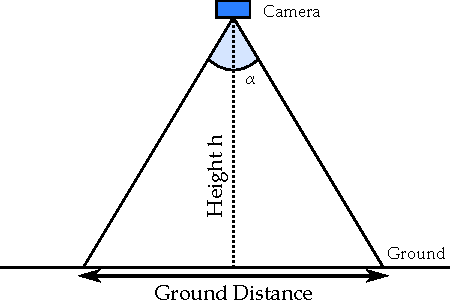
\includegraphics[width=0.65\textwidth]{figures/Orbiter/imaging_angle_of_view}
\caption{Definition of the angle of view. Adapted from:\cite{dsil2014}.}
\label{fig:angle_of_view_def}
\end{figure}
From this figure, it can be seen how the tangent of half the angle of view is equal to the half the ratio between the ground distance and the height. This applies to both the horizontal and vertical distance. If the sensor is not square, the angle and therefore the distance will be different.
\begin{equation}
\label{eq:angle_of_view}
\tan{\frac{\alpha_x}{2}} = \frac{x}{2h}
\end{equation}
By arranging the two equations, the ground distance is defined:
\begin{equation}
\label{eq:ground_dist}
dist_x = 2h\cdot \tan{\frac{\alpha_x}{2}}
\end{equation}
The ground distance defines the total distance covered, when the contributions from all pixels are added together. Therefore, the ground distance per pixel ($\mu_x$ or $\mu_y$)is easily found when the sensor resolution is known. This can be seen in equation \eqref{eq:ground_dist_pixel}:
\begin{equation}
\label{eq:ground_dist_pixel}
\mu_x = \frac{x}{r_x} = 2h\cdot \tan{\frac{\alpha_x}{2}}
\end{equation}
By solving for the the field of view using \eqref{eq:ground_dist}, the focal length can be found using equation \eqref{eq:focal_len_fieldofview}. This applies to both the horizontal and vertical direction, if the sensor is not square.
\begin{equation}
\label{eq:angle_of_view_ground_dist}
\alpha_x = 2h\cdot \tan{\frac{dist_x}{2}}
\end{equation}
The focal length can then be calculated by solving for the focal length in equation \eqref{eq:focal_length_angle_of_view} and using the horizontal or vertical sensor size as $d$.
\begin{equation}
\label{eq:focal_length_angle_of_view}
f = 0.5\cdot\frac{d}{\tan{\left(0.5\cdot \alpha\right)}}
\end{equation}
%\subsection{Camera Basics}
%\todo[inline]{pinhole camera basics}
%\todo[inline]{ccd, cmos difference}
%\subsection{Telescope Systems}
%\todo[inline]{Types of imagers etc.}
%\section{Spectroscopy}
%\todo[inline]{See power point presentation}
%\section{Europa Surface Environment}
%\todo[inline]{Moon Environment (Radiation etc)}
%\section{Calibrating the Geo-localization System}
%\todo[inline]{How to calibrate (point at Jupiter, get transfer matrix using star trackers)}
%\section{Protecting from radiation}
%\todo[inline]{How to protect from radiation. Dynamic Response to Radiation (Julia)}
%\section{High Gate Measurement}
%\todo[inline]{High Gate Measurement (Operating at very far distance, to track trajectory)}